%%%% 第一版 2020.10
%此文档为普通物理实验三林伟华老师要求的物理实验报告模板
%作者:武汉大学物理科学与技术学院18级詹睿知
%参考自电子信息学院实验报告模板
%%%% 第二版 2022.8
%更改优化了documentclass
\documentclass{WHUReport}
\usepackage[]{amsmath}
\usepackage{natbib}
\setcitestyle{numbers,square}
\usepackage{diagbox} %斜线表头

%%%% 以下填写学生信息及实验题目
\newcommand{\major}{物理学}
\newcommand{\name}{郑卜凡}
\newcommand{\stuid}{2021302022016}
\newcommand{\Name}{Bufan Zheng}
\newcommand{\course}{普通物理实验三}
\newcommand{\newtitle}{密里根油滴实验测定电子电荷量}
\newcommand{\Title}{Determining the Charge of the Electron by Millikon Oil Drop Experiment}

\begin{document}
\pagestyle{maincontent} 
%\bibliographystyle{plain}

\begin{center}
\zihao{-2} \textbf{\newtitle}\\
\zihao{7}~\\
\zihao{4} \kaishu \name \ \ (\stuid)\\
\zihao{5} \kaishu (武汉大学物理科学与技术学院,湖北省 武汉市 430072)\\
\end{center}
\zihao{-5}\textbf{摘\quad 要:}
%在此处修改中文摘要
本实验利用CCD显微密里根油滴实验测定了电子电荷量,利用作图法处理数据,最终结果相对误差控制在1\%左右,并对实验原理和实验误差进行了细致的分析。\\
\zihao{-5}\textbf{关键词:}电子;元电荷;密立根油滴实验;误差分析
~\\
\begin{center}
	\zihao{3}\textbf{\Title}\\
	\zihao{-4} \Name\quad (\stuid)\\
	\zihao{5} School of physical science and technology, Wuhan University, Wuhan, 430072, China
\end{center}

\zihao{5}\textbf{Abstract:}In this work, the charge of the electron was measured by Millikan oil drop experiment. Using the graphic method to process the experimental data, the relative error was controlled at about 1\%, the principle and error of the experiment has also been analyzed.

\zihao{5}\textbf{Keywords: }electron; charge of the electron; Millikan oil drop experiment; error analysis

\begin{multicols}{2}
	电子电荷量是物理学中非常重要的基本常量,最早是由美国著名物理学家Robert A.Millikan经过十多年设计实验并完成测定的\upcite{ref1}。这一实验设计思想简明巧妙,但结论却具有不容置疑的说服力,因此堪称物理实验的精华和典范\upcite{ref2}。1908年,在总结前人实验经验的基础上,密立根开始研究带电液滴在电场中的运动过程。结果表明,液滴上的电荷是某一基本电荷的整数倍,但测量结果十分不准确,两年后他用油滴代替易挥发的水滴成功用实验证明了电荷的不连续性,再次证明了电子的存在,且实验结果与目前世界公认值仅相差1\%。密立根精彩的实验工作使他得到了1923年Nobel物理学奖。
	
	本次实验采用CCD摄像机和监视仪,可以非常清楚地看到钟表油油滴的运动过程,大大改善了实验条件,能更加清楚的了解实验原理。
	\section{实验原理}
	实验的基本思想是使带电油滴在两金属板之间处于受力平衡状态,按照运动方式分类,可以分为平衡法和动态法两种测量方式\upcite{ref3}。本次实验使用平衡法进行测量,基本思想是先让油滴静止在电场中的某处,然后再让其在重力场中自由下落。
	\subsection{动态法}
	在重力场中自由下落的小油滴会受到重力空气浮力和空气阻力的作用,根据Stokes定律可以写下平衡方程为:
	\begin{equation}\label{1}
		m_1 g-m_2g=Kv_f
	\end{equation}
	这里$m_2$为排开空气质量。但是直接测量$m_1,m_2$是困难的,可以考虑用油滴和空气的密度$\rho_1,\rho_2$进行代替,即:
	\begin{equation}\label{2}
		m_1 g-m_2g=\frac{4}{3}\pi r^3(\rho_1-\rho_2)g
	\end{equation}
	根据Stokes定律,$K=6\pi\eta r$,代入\ref{1}和\ref{2}可以解出:
	\begin{equation}\label{3}
		v_f=\frac{2gr^2}{9\eta}(\rho_1-\rho_2)
	\end{equation}
	因此液滴半径可以表示为:
	\begin{equation}
		r=\left[\frac{9\eta v_f}{2g(\rho_1-\rho_2)}\right]^{\frac{1}{2}}
	\end{equation}
	考虑到油滴的大小与空气分子间隙相当,空气已经不能看作是连续介质,其空气粘度$\eta$需要用下式进行修正:
	\begin{equation}
		\eta^\prime=\frac{\eta}{1+\frac{b}{pr}}
	\end{equation}
	其中$p$为气压,$b\approx 0.00823\operatorname{N/m}$,因此\ref{3}需要修正为:
	\begin{equation}
		v_f=\frac{2gr^2}{9\eta}(\rho_1-\rho_2)(1+\frac{b}{pr})
	\end{equation}
	再考虑在与重力相反方向的匀强电场$E$作用下,油滴的匀速上升,平衡方程可以写为:
	\begin{equation}
		qE=(m_1-m_2)g+Kv_r
	\end{equation}
	联合前面几个式子可以解得:
	\begin{equation}\label{key}
		q=9\sqrt{2}\pi\left[\frac{\eta^3}{(\rho_1-\rho_2)g}\right]^{\frac{1}{2}}\frac{1}{E}\left(1+\frac{v_r}{v_f}\right){v_f}^{\frac{3}{2}}\left[\frac{1}{1+\frac{b}{pr}}\right]^{\frac{3}{2}}
	\end{equation}
	实验中可以固定油滴运动的距离$s$,然后除去运动时间$t$求得运动速度,并且电场强度根据所加电压与仪器平行板之间距离比值$U/d$确定,因此,式\ref{key}可以写成下面得形式:
	\begin{equation}
		\begin{aligned}
			q=9\sqrt{2}\pi d&\left[\frac{(\eta s)^3}{(\rho_1-\rho_2)g}\right]^{\frac{1}{2}}\frac{1}{U}\left(\frac{1}{t_f}+\frac{1}{t_r}\right)\left(\frac{1}{t_f}\right)^{\frac{1}{2}}\\\times&\left[\frac{1}{1+\frac{b}{pr}}\right]^{\frac{3}{2}}
		\end{aligned}
	\end{equation}
	其中前面的因子是与实验本身无关的固定常数,合称为$C$,即仪器参数,则上式可以简化为:
	\begin{equation}\label{key2}
		q=C\frac{1}{U}\left(\frac{1}{t_f}+\frac{1}{t_r}\right)\left(\frac{1}{t_f}\right)^{\frac{1}{2}}\left[\frac{1}{1+\frac{b}{pr}}\right]^{\frac{3}{2}}
	\end{equation}
	本实验所用仪器的仪器参数$C\approx 1.0226\times10^{-14}\operatorname{kg\cdot m^2/\sqrt{s}}$。
	\subsection{平衡法}
	平衡法唯一的不同是首先调节电压让液滴在匀强电场中受力平衡,即:
	\begin{equation}
		qE=(m_1-m_2)g
	\end{equation}
	然后再让油滴在重力场中自由下落,推导和前面动态法一致,只是现在$v_r=0$,那么式\ref{key2}中取$1/t_r=0$便得到平衡法测量时电荷的计算方式:
	\begin{equation}\label{12}
		q=C\frac{1}{U}\left(\frac{1}{t_f}\right)^{\frac{3}{2}}\left[\frac{1}{1+\frac{b}{pr}}\right]^{\frac{3}{2}}
	\end{equation}
	\subsection{元电荷的测量方法}
	测量油滴上所带电荷量$q$的目的是找出电荷的最小单位有计算法和作图法两种方式\upcite{ref5}:
	\subsubsection{计算法}
	至少测量5个油滴,记录每个油滴的带电量$q_i$,再根据$\frac{q_i}{e_0}$取整后求得每个油滴所带电子个数,其中$e_0\approx 1.602\times 10^{-19}\operatorname{C}$为国际公认测量值。再根据$q_i/n_i$得到每次测量的基本电荷,最后取平均值即为最终测量结果。
	\subsubsection{作图法}
	得到$q_i$和对应的$n_i$后,以$q$为纵坐标,$n$为横坐标作图,拟合得到的直线斜率便为基本电荷$e$。
	\section{实验内容与步骤}
	\subsection{仪器调整}
	\subsubsection{水平调整}
	利用调平螺钉和水平仪将仪器调平,这一步是为了让带点平板与重力方向垂直,这样产生的电场才与重力方向平行,使得测量过程中带点油滴不会发生左右的漂移。
	\subsubsection{喷雾器调整}
	将少量钟表油缓慢地倒入喷雾器的储油腔内,使钟表油湮没提油管下方,油不要太多,以免实验过程中不慎将油倾倒至油滴盒内堵塞落油孔。将喷雾器竖起,用手挤压气囊,使得提油管内充满钟表油。
	\subsubsection{CCD成像系统调整}
	打开进油量开关,从喷雾口喷入油雾,此时监视器上应该出现大量运动油滴的像。若没有看到油滴的像,则需调整调焦旋钮或检查喷雾器是否有油雾喷出。
	\subsection{油滴选择}
	选择合适的油滴是影响实验精确度的关键因素。若油滴过小,布朗运动比较明显不易控制,油滴过大又会导致下落过快,从而时间测量的相对误差增大,而且油滴带多个电子的概率大大增加,这样不易确定油滴所带的电子个数。
	
	文献\cite{ref4}中详细分析了油滴应当如何选取,文献指出,选取油滴的半径在$0.7\operatorname{\mu m}\sim 1.3\operatorname{\mu m}$之间是最合适的,选取方法可以通过先去掉外部电压,让油滴自由下落大约$2\operatorname{mm}$,如果下落时间在$10\operatorname{s}\sim 30\operatorname{s}$左右,则所选油滴非常合适,本次实验将尽可能的遵循这一原则选取油滴。
	\subsection{实验步骤}
	本次实验使用平衡法进行测量,比较容易操作,实验步骤如下:
	\begin{itemize}
		\item[1.] 开启电源,进入实验界面将工作状态案件切换至“工作”,红色指示灯点亮,将“平衡/提升”按键置于“平衡”。
		\item[2.] 平衡电压调整为$200\operatorname{V}$左右,这样是为了后面选取合适的油滴,不同的电压初始设定会筛选出不同的油滴,经验表明调整为$200\operatorname{V}$左右选出的油滴比较适合实验。通过喷雾口喷入油雾,此时监视器上出现大量运动油滴,根据前面的方式调整平衡电压选取合适的油滴 ,再利用“提升”按键将其平衡在最上面的格线上。
		\item[3.] 将“$0\operatorname{V}$/工作”按键置于“$0\operatorname{V}$”,让油滴自然下落,下落到$0$标记线处立即开始计时,下落到$1.6$标记线处时停止计时,按下“确认”键记录数据。
		\item[4.] 将“平衡/提升”按键置于“提升”,将油滴重新平衡在最上方格线上,重新调节平衡电压(如果需要的话),如果平衡电压发生了突变说明油滴失去了电子,需要重新进行实验。
		\item[5.] 重复前面的步骤测量五组数据,系统会自动利用公式\ref{12}进行计算,表达结果。
		\item[6.] 寻找新的油滴重复实验。
	\end{itemize}
	\section{实验数据处理及结果表达}
	本次实验共仔细挑选了六个油滴进行实验,测得实验数据如下图:
	\begin{figure}[H]
		\centering
		\includegraphics[width=0.8\linewidth]{figs/1.jpg}
		\caption{第一组}
	\end{figure}
	\begin{figure}[H]
		\centering
		\includegraphics[width=0.8\linewidth]{figs/2.jpg}
		\caption{第二组}
	\end{figure}
	\begin{figure}[H]
		\centering
		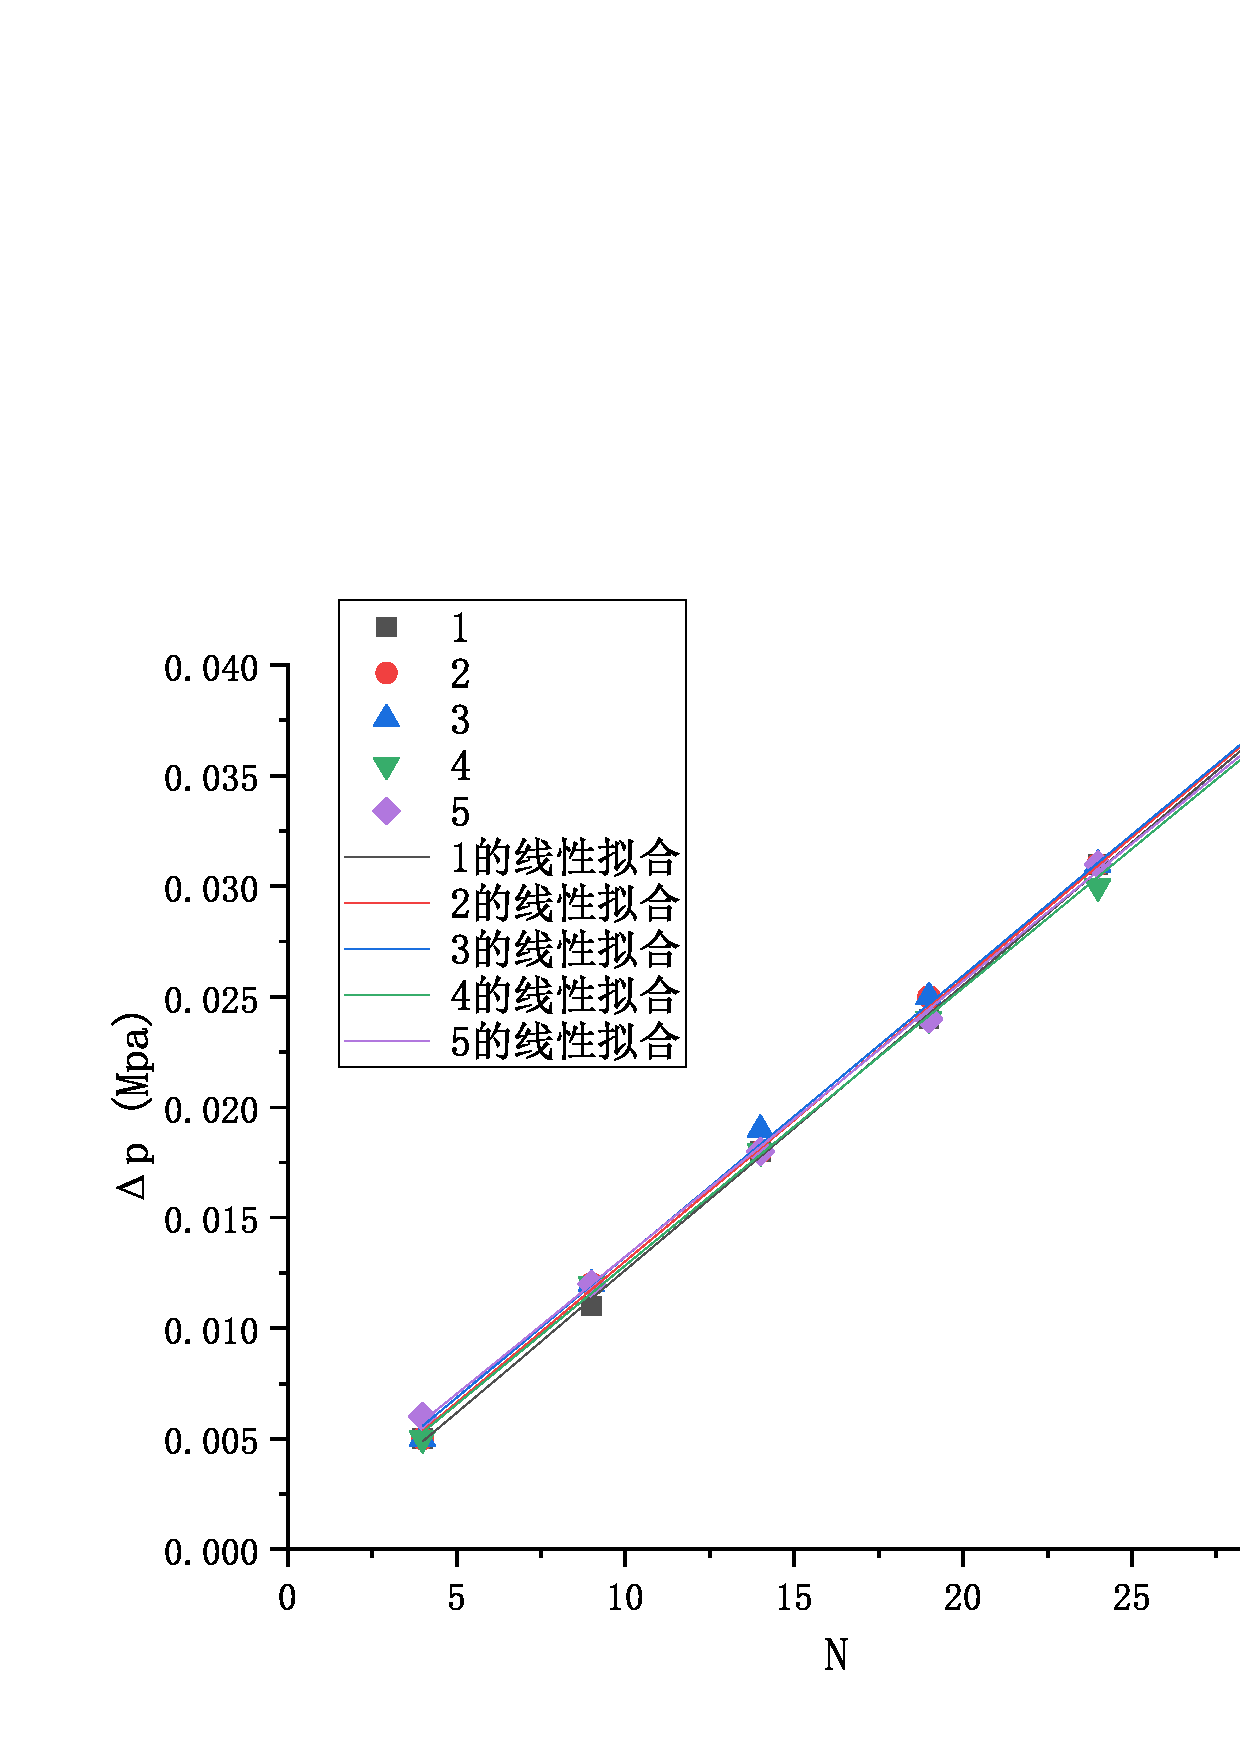
\includegraphics[width=0.8\linewidth]{figs/3.jpg}
		\caption{第三组}
	\end{figure}
	\begin{figure}[H]
		\centering
		\includegraphics[width=0.8\linewidth]{figs/4.jpg}
		\caption{第四组}
	\end{figure}
	\begin{figure}[H]
		\centering
		\includegraphics[width=0.8\linewidth]{figs/5.jpg}
		\caption{第五组}
	\end{figure}
	\begin{figure}[H]
		\centering
		\includegraphics[width=0.8\linewidth]{figs/6.jpg}
		\caption{第六组}
	\end{figure}
	根据上面的数据利用计算法处理数据得到下表:
	\begin{table}[H]
		\centering
		\resizebox{0.97\linewidth}{2.3em}{
		\begin{tabular}{|l|c|c|c|c|c|c|}
			\hline
			$q_i(\operatorname{\times 10^{-19}C})$ & 1.665 & 5.069 & 5.114 & 8.089 & 11.477 & 27.619 \\ \hline
			$n_i$                                  & 1     & 3     & 3     & 5     & 7      & 17     \\ \hline
			$e_i(\operatorname{\times 10^{-19}C})$ & 1.665 & 1.690 & 1.705 & 1.617 & 1.639  & 1.625  \\ \hline
		\end{tabular}}
		\caption{实验数据表}
	\end{table}
	第三组实验数据明显相较于其它几组偏大,偶然误差较大,所以可以将其从实验数据中剔除,利用剩下五组数据求得结果为:
	\begin{equation}
		e = (1.647\pm0.030 )\times 10^{-19}\operatorname{C}
	\end{equation}
	相对不确定度为$1.8\%$,与真值$e_0$之间的相对误差约为$2.8\%$。
	
	根据上表还可以绘制出$q\mbox{-}n$点图的拟合直线为:
	\begin{figure}[H]
		\centering
		\includegraphics[width=\linewidth]{figs/fit.pdf}
		\caption{拟合曲线}
	\end{figure}
	根据Origin软件的拟合结果,我们得到作图法得到的结果为:
	\begin{equation}
		e = (1.619\pm0.008 )\times 10^{-19}\operatorname{C}
	\end{equation}
	拟合相对不确定度为$0.5\%$,与真值$e_0$之间的相对误差约为$1.1\%$。
	
	不难发现,用作图法处理数据相较于计算法不确定度更小,结果更加可靠,而且得到的结果与真值之间的相对误差更小,实验结果更加精确,与国际公认测量值之间的误差仅有$1\%$,真正复现了密立根所做实验,他当时的实验测定值与真值相对误差正是约$1\%$!
	\section{实验误差分析}
	本实验中最重要的因素是油滴的选取,油滴上所带的电荷量以及油滴的大小都是极其重要的因素,所以进行实验前一定要反复利用文献\cite{ref4}中方法进行预实验确定油滴品质好坏。实验中测量结果均偏大,从公式\ref{12}发现是$t_f$或者$U$测量偏小,$U$测量误差主要是平衡时由于空气的对流以及布朗运动导致平衡不易使用肉眼判断,而且实验仪器的$U$最小调节单位为$1\operatorname{V}$,无法更加精确调节,只能通过多次实验减小偶然误差。
	
	$t_f$的测量误差有很多因素,实验仪是否水平决定下落距离$s$是否为$1.6\operatorname{mm}$,调平不够精确会使得$s$偏小,导致测量结果偏小。由于空气的对流和布朗运动也导致了油滴本身并不是严格的匀速直线运动,这可以通过尽量在保证油滴带电量比较小的情况下选取更大半径的油滴进行实验来减小误差,文中已提及如何达到这一点。另外,由于油滴从某一高度下落在空气阻力的作用下达到匀速运动是需要时间的,所以实验中我们先让油滴平衡在最上面的格线上,而不是直接平衡在$0$标记线处,这样才能保证开始计时时油滴接近于匀速运动。实验者计时的反应时间和仪器本身的反应时间也是一个因素,所以需要多次测量。
	\section{结\quad 论}
	本次实验利用CCD显微密里根油滴实验仪利用“平衡法”对电子电荷量进行了测量,测量结果误差仅有1.1\%,作为大学物理教学实验已经是很好的结果。处理实验数据时,使用作图法和计算法两种常用实验数据处理技术,并对两种方法的好坏进行了对比分析。通过此次实验对密立根实验的原理有了深刻的理解,并探究了实验误差产生的原因所在,并提出了一些可行的解决思路。对科学史上著名的实验,特别是这种诺贝尔奖级别的优雅实验进行亲自操作,对于物理学史本身和前人的探索过程也有了一些“感同身受”的独特理解。
	\bibliographystyle{unsrt}
	\begin{thebibliography}{99}  
		\bibitem{ref1}刘战存,李萍萍.密立根对电子电荷的测定和对光电效应的实验研究[J].大学物理,2001(11):43-46.DOI:10.16854/j.cnki.1000-0712.2001.11.014.
		\bibitem{ref2}陈思羽,赵春然.密立根与密立根油滴实验——纪念密立根获诺贝尔物理学奖100周年[J].物理教师,2023,44(05):77-80.
		\bibitem{ref3}邱成锋,杨嘉,张金凤.密里根油滴实验中两种方法分析平衡电压和下落时间选取[J].大学物理实验,2014,27(02):56-58.DOI:10.14139/j.cnki.cn22-1228.2014.02.001.
		\bibitem{ref4}陆佩.密立根油滴实验中影响油滴控制的因素分析及对策[J].大学物理实验,2007(03):14-16.
		\bibitem{ref5}郑雪丽,李巧梅,杨骏骏等.多种方法结合处理密立根油滴实验数据[J].物理与工程,2019,29(S1):119.
	\end{thebibliography}
\end{multicols}

\end{document}
